\documentclass[border=3pt,tikz]{standalone}
\usepackage{amsmath,amssymb}
\usepackage{newtxtext,newtxmath}
\usetikzlibrary{arrows.meta,calc,decorations.pathmorphing}

%% Fig. 1: axisymmetric wire drawing, boundaries S1--S5 and the die geometry.
%% Schematic, not to scale: the reduction and the bearing are exaggerated.
\definecolor{sfive}{RGB}{46,160,67}
\definecolor{sfour}{RGB}{240,180,0}
\definecolor{sthree}{RGB}{31,90,220}
\definecolor{stwo}{RGB}{220,30,30}

\begin{document}
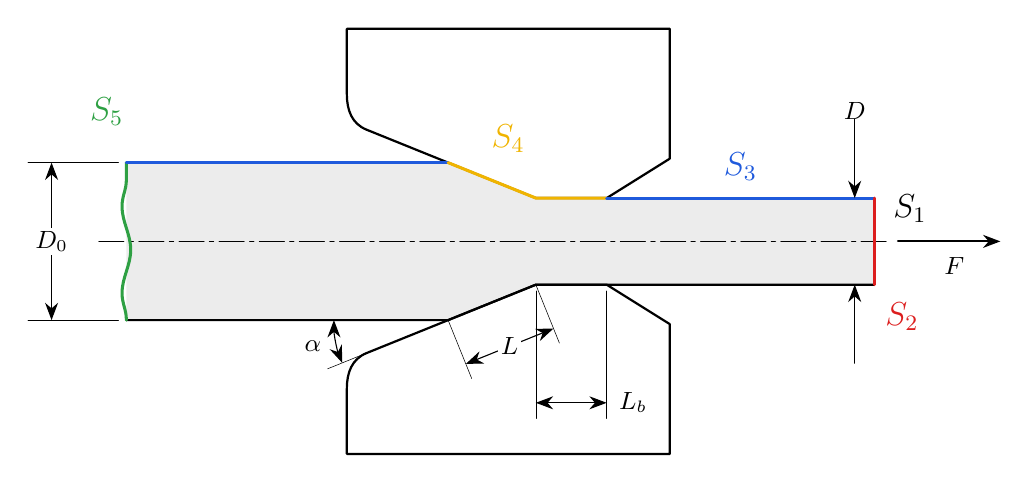
\begin{tikzpicture}[
  font=\small, line cap=round, line join=round,
  >={Stealth[length=2.2mm]},
  dim/.style ={thin, <->},
  ext/.style ={very thin},
  bnd/.style ={line width=1.1pt},
  die/.style ={draw, thick, fill=white},
]
%% geometry (cm): R0 = 1, R = 0.55, cone ends at xb, bearing to xe
\def\Rz{1.00}\def\Rf{0.55}
\def\xb{5.70}\def\xe{6.60}\def\tna{0.404}   % tan of the drawn semi-angle (22 deg)
\def\xin{0.50}\def\xout{10.0}\def\xd{3.30}\def\xr{7.40}\def\ytop{2.70}
\pgfmathsetmacro{\xc}{\xb-(\Rz-\Rf)/\tna}     % wire meets the cone
\pgfmathsetmacro{\yd}{\Rf+(\xb-\xd)*\tna}     % cone meets the die face

%% wire
\fill[gray!15] (\xin,-\Rz) -- (\xc,-\Rz) -- (\xb,-\Rf) -- (\xout,-\Rf)
  -- (\xout,\Rf) -- (\xb,\Rf) -- (\xc,\Rz) -- (\xin,\Rz) -- cycle;

%% die, upper and lower halves
\foreach \s in {1,-1}{
  \draw[die] (\xd,\s*\ytop) -- (\xr,\s*\ytop) -- (\xr,\s*1.05) -- (\xe,\s*\Rf)
    -- (\xb,\s*\Rf) -- ($(\xd,\s*\yd)+(0.25,-\s*0.25*\tna)$)
    to[out=180-\s*22,in=-\s*90] (\xd,\s*\yd+\s*0.35) -- cycle;
}

%% axis of symmetry
\draw[thin, dash pattern=on 9pt off 2pt on 1.5pt off 2pt] (0.15,0) -- (\xout+0.15,0);

%% lower contour of the wire in black
\draw[thick] (\xin,-\Rz) -- (\xc,-\Rz) -- (\xb,-\Rf) -- (\xout,-\Rf);

%% boundaries of the upper half
\draw[bnd, sfive, decorate, decoration={snake, amplitude=0.55mm, segment length=11mm}]
  (\xin,-\Rz) -- (\xin,\Rz);
\draw[bnd, sthree] (\xin,\Rz) -- (\xc,\Rz);
\draw[bnd, sfour]  (\xc,\Rz) -- (\xb,\Rf) -- (\xe,\Rf);
\draw[bnd, sthree] (\xe,\Rf) -- (\xout,\Rf);
\draw[bnd, stwo]   (\xout,-\Rf) -- (\xout,\Rf);

\node[sfive,  font=\large] at (0.25,1.65) {$S_5$};
\node[sfour,  font=\large] at (5.35,1.30) {$S_4$};
\node[sthree, font=\large] at (8.30,0.95) {$S_3$};
\node[stwo,   font=\large] at (10.35,-0.95) {$S_2$};
\node[font=\large]         at (10.45,0.42) {$S_1$};

%% drawing force
\draw[->, thick] (\xout+0.3,0) -- (\xout+1.6,0) node[pos=0.55, below=2pt] {$F$};

%% D0
\draw[ext] (\xin-0.10,\Rz) -- (-0.75,\Rz);
\draw[ext] (\xin-0.10,-\Rz) -- (-0.75,-\Rz);
\draw[dim] (-0.45,-\Rz) -- (-0.45,\Rz);
\node[fill=white, inner sep=1.2pt] at (-0.45,0) {$D_0$};

%% D
\draw[ext] (\xout-0.25,\Rf+0.05) -- (\xout-0.25,1.55);
\draw[ext] (\xout-0.25,-\Rf-0.05) -- (\xout-0.25,-1.55);
\draw[->, thin] (\xout-0.25,1.35) -- (\xout-0.25,\Rf);
\draw[->, thin] (\xout-0.25,-1.35) -- (\xout-0.25,-\Rf);
\node at (\xout-0.25,1.65) {$D$};

%% L along the lower cone, offset into the die
\coordinate (c1) at (\xc,-\Rz);
\coordinate (c2) at (\xb,-\Rf);
%% offsets normal to the cone, away from the wire (into the die)
\draw[ext] (c1) -- ($(c1)!0.80cm!-90:(c2)$);
\draw[ext] (c2) -- ($(c2)!0.80cm!90:(c1)$);
\draw[dim] ($(c1)!0.60cm!-90:(c2)$) -- ($(c2)!0.60cm!90:(c1)$)
  node[midway, fill=white, inner sep=1pt] {$L$};

%% L_b under the lower bearing
\draw[ext] (\xb,-\Rf-0.08) -- (\xb,-2.25);
\draw[ext] (\xe,-\Rf-0.08) -- (\xe,-2.25);
\draw[dim] (\xb,-2.05) -- (\xe,-2.05);
\node[right=1pt] at (\xe,-2.05) {$L_b$};

%% semi-angle between the wire surface and the cone
\draw[ext] (c1) -- ($(c1)!-1.65cm!(c2)$);
\draw[ext] (c1) -- ++(-1.75,0);
\draw[thin, <->] ($(c1)+(-1.45,0)$) arc[start angle=180, end angle={180+atan(\tna)}, radius=1.45];
\node at ($(c1)+({180+atan(\tna)/2}:1.75)$) {$\alpha$};
\end{tikzpicture}
\end{document}
